\begin{figure}[t]
\centering
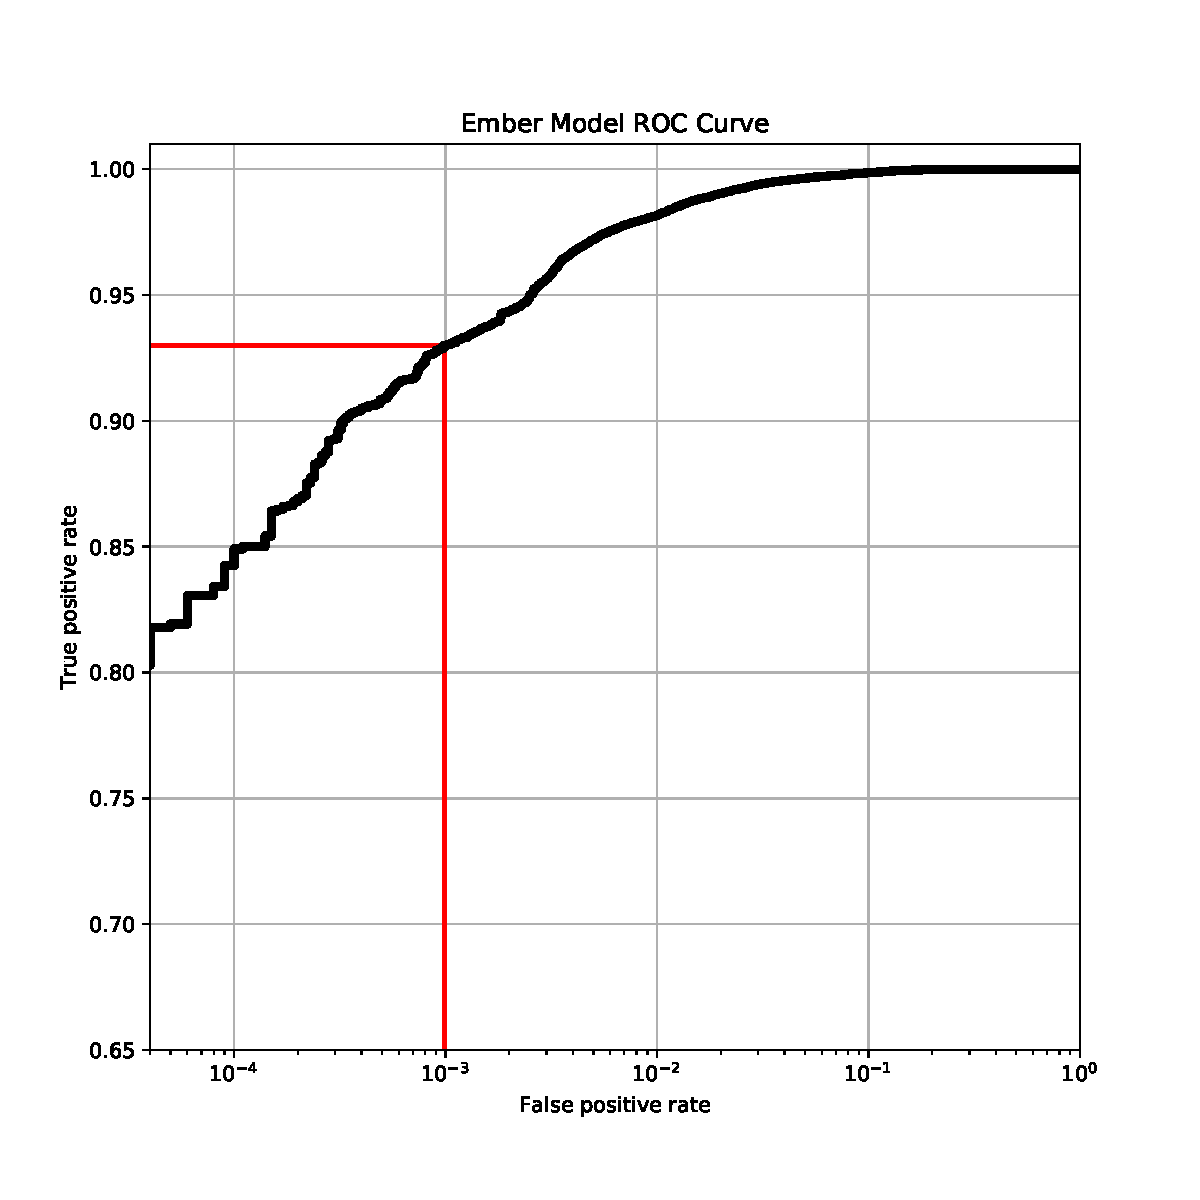
\includegraphics[width=3.8in]{figs/ROC.pdf}
\caption{ROC curve with log scale for false positive rate (FPR). The threshold shown (red) corresponds to a 0.1\% FPR and a detection rate about 93\%.  At 1\% FPR the detection rate exceeds 98\%.\label{fig:roc}}
\end{figure}

\begin{figure}[t]
\centering
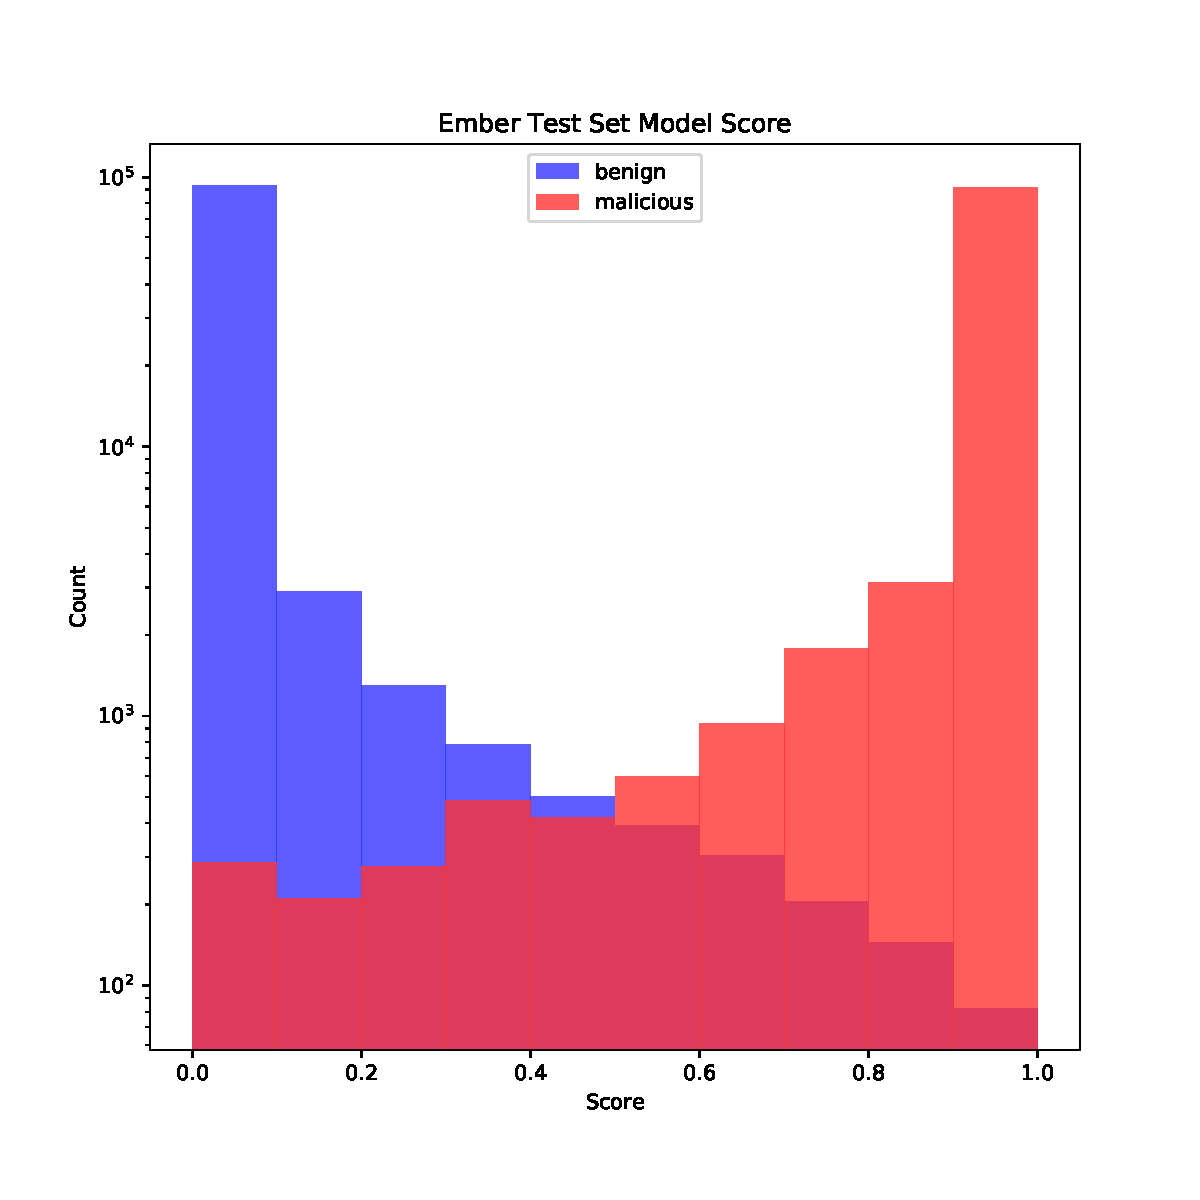
\includegraphics[width=3.8in]{figs/test_set_score.pdf}
\caption{Distribution of model test scores on the test set (note the logarithmic scale)\label{fig:scores}}
\end{figure}

EMBER includes code that demonstrates how to use the raw features in the training set (labeled samples only) for building a supervised learning model, which we provide as a baseline model. The model building process consists of vectorizing the raw features (each object into a vector of dimension 2351), using the feature hashing trick where necessary, as described previously.  On a 2015 MacBook Pro i7, it took 20 hours to vectorize the raw features into model features.  From the vectorized features, we trained a gradient-boosed decision tree (GBDT) model using \texttt{LightGBM} with default parameters (100 trees, 31 leaves per tree), resulting in fewer than 10K tunable parameters \cite{ke2017lightgbm}. Model training took 3 hours. Baseline model performance may be much improved with appropriate hyper-parameter optimization, which is of less interest to us in this work.

A ROC curve of the resulting model is shown in Figure \ref{fig:roc}, and a distribution of scores for malicious and benign samples in the test set is shown in Figure \ref{fig:scores}.  The ROC AUC exceeds 0.99911.  A threshold of 0.871
on the model score results in less than 0.1\% FP rate at a detection rate exceeding 92.99\%.  At less than 1\% FP rate, the model exceeds 98.2\% detection rate.

As discussed in Section \ref{sec:background}, it has been suggested that owing to the dataset it was trained on, the Adobe Malware Classifier is biased towards non-Windows vs. Windows classification, rather than a true malicious vs. benign problem \cite{seymour2016howto}.  We evaluated the pre-trained J48 model on our test set and found that it exhibits an alarming 53\% false positive rate and an 8\% false negative rate.  This would seem to substantiate previous claims about dataset bias. However, whether this poor performance can be ascribed to stale training data or dataset bias or both is out of the scope of this paper.  But clearly, it is an inappropriate baseline model.

As a comparative study, we trained MalConv \cite{raff2017malware} on the raw binaries underlying the dataset.  We used the model architecture and training setup as prescribed and verified by the authors, except that we train with a batch size of 100 instead of 256 due to GPU memory constraints.  We trained using data parallelism across two Titan X (Pascal) GPUs.  Each epoch took 25 hours, and we trained for 10 epochs (10 days).  The resulting model has roughly 1M parameters.  Applied to the raw binaries corresponding to the EMBER test set, the Malconv ROC AUC is 0.99821, corresponding to a 92.2\% detection rate at a false positive rate less than 0.1\%, or a 97.3\% detection rate at a less than 1\% false positive rate.  This is slightly lower performance than using \texttt{LightGBM} with no hyper-parameter tuning.  Evidently, despite increased model size and computational burden, featureless deep learning models have yet to eclipse the performance of models that leverage domain knowledge via parsed features.
